\documentclass[1p]{elsarticle_modified}
%\bibliographystyle{elsarticle-num}

%\usepackage[colorlinks]{hyperref}
%\usepackage{abbrmath_seonhwa} %\Abb, \Ascr, \Acal ,\Abf, \Afrak
\usepackage{amsfonts}
\usepackage{amssymb}
\usepackage{amsmath}
\usepackage{amsthm}
\usepackage{scalefnt}
\usepackage{amsbsy}
\usepackage{kotex}
\usepackage{caption}
\usepackage{subfig}
\usepackage{color}
\usepackage{graphicx}
\usepackage{xcolor} %% white, black, red, green, blue, cyan, magenta, yellow
\usepackage{float}
\usepackage{setspace}
\usepackage{hyperref}

\usepackage{tikz}
\usetikzlibrary{arrows}

\usepackage{multirow}
\usepackage{array} % fixed length table
\usepackage{hhline}

%%%%%%%%%%%%%%%%%%%%%
\makeatletter
\renewcommand*\env@matrix[1][\arraystretch]{%
	\edef\arraystretch{#1}%
	\hskip -\arraycolsep
	\let\@ifnextchar\new@ifnextchar
	\array{*\c@MaxMatrixCols c}}
\makeatother %https://tex.stackexchange.com/questions/14071/how-can-i-increase-the-line-spacing-in-a-matrix
%%%%%%%%%%%%%%%

\usepackage[normalem]{ulem}

\newcommand{\msout}[1]{\ifmmode\text{\sout{\ensuremath{#1}}}\else\sout{#1}\fi}
%SOURCE: \msout is \stkout macro in https://tex.stackexchange.com/questions/20609/strikeout-in-math-mode

\newcommand{\cancel}[1]{
	\ifmmode
	{\color{red}\msout{#1}}
	\else
	{\color{red}\sout{#1}}
	\fi
}

\newcommand{\add}[1]{
	{\color{blue}\uwave{#1}}
}

\newcommand{\replace}[2]{
	\ifmmode
	{\color{red}\msout{#1}}{\color{blue}\uwave{#2}}
	\else
	{\color{red}\sout{#1}}{\color{blue}\uwave{#2}}
	\fi
}

\newcommand{\Sol}{\mathcal{S}} %segment
\newcommand{\D}{D} %diagram
\newcommand{\A}{\mathcal{A}} %arc


%%%%%%%%%%%%%%%%%%%%%%%%%%%%%5 test

\def\sl{\operatorname{\textup{SL}}(2,\Cbb)}
\def\psl{\operatorname{\textup{PSL}}(2,\Cbb)}
\def\quan{\mkern 1mu \triangleright \mkern 1mu}

\theoremstyle{definition}
\newtheorem{thm}{Theorem}[section]
\newtheorem{prop}[thm]{Proposition}
\newtheorem{lem}[thm]{Lemma}
\newtheorem{ques}[thm]{Question}
\newtheorem{cor}[thm]{Corollary}
\newtheorem{defn}[thm]{Definition}
\newtheorem{exam}[thm]{Example}
\newtheorem{rmk}[thm]{Remark}
\newtheorem{alg}[thm]{Algorithm}

\newcommand{\I}{\sqrt{-1}}
\begin{document}

%\begin{frontmatter}
%
%\title{Boundary parabolic representations of knots up to 8 crossings}
%
%%% Group authors per affiliation:
%\author{Yunhi Cho} 
%\address{Department of Mathematics, University of Seoul, Seoul, Korea}
%\ead{yhcho@uos.ac.kr}
%
%
%\author{Seonhwa Kim} %\fnref{s_kim}}
%\address{Center for Geometry and Physics, Institute for Basic Science, Pohang, 37673, Korea}
%\ead{ryeona17@ibs.re.kr}
%
%\author{Hyuk Kim}
%\address{Department of Mathematical Sciences, Seoul National University, Seoul 08826, Korea}
%\ead{hyukkim@snu.ac.kr}
%
%\author{Seokbeom Yoon}
%\address{Department of Mathematical Sciences, Seoul National University, Seoul, 08826,  Korea}
%\ead{sbyoon15@snu.ac.kr}
%
%\begin{abstract}
%We find all boundary parabolic representation of knots up to 8 crossings.
%
%\end{abstract}
%\begin{keyword}
%    \MSC[2010] 57M25 
%\end{keyword}
%
%\end{frontmatter}

%\linenumbers
%\tableofcontents
%
\newcommand\colored[1]{\textcolor{white}{\rule[-0.35ex]{0.8em}{1.4ex}}\kern-0.8em\color{red} #1}%
%\newcommand\colored[1]{\textcolor{white}{ #1}\kern-2.17ex	\textcolor{white}{ #1}\kern-1.81ex	\textcolor{white}{ #1}\kern-2.15ex\color{red}#1	}

{\Large $\underline{12n_{0814}~(K12n_{0814})}$}

\setlength{\tabcolsep}{10pt}
\renewcommand{\arraystretch}{1.6}
\vspace{1cm}\begin{tabular}{m{100pt}>{\centering\arraybackslash}m{274pt}}
\multirow{5}{120pt}{
	\centering
	\includegraphics[width=112pt]{../../../GIT/diagram.site/Diagrams/png/2903_12n_0814.png}\\
\ \ \ A knot diagram\footnotemark}&
\allowdisplaybreaks
\textbf{Linearized knot diagam} \\
\cline{2-2}
 &
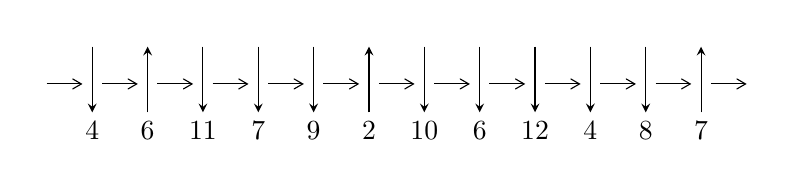
\begin{tikzpicture}[x=20pt, y=17pt]
	% nodes
	\node (C0) at (0, 0) {};
	\node (C1) at (1, 0) {};
	\node (C1U) at (1, +1) {};
	\node (C1D) at (1, -1) {4};

	\node (C2) at (2, 0) {};
	\node (C2U) at (2, +1) {};
	\node (C2D) at (2, -1) {6};

	\node (C3) at (3, 0) {};
	\node (C3U) at (3, +1) {};
	\node (C3D) at (3, -1) {11};

	\node (C4) at (4, 0) {};
	\node (C4U) at (4, +1) {};
	\node (C4D) at (4, -1) {7};

	\node (C5) at (5, 0) {};
	\node (C5U) at (5, +1) {};
	\node (C5D) at (5, -1) {9};

	\node (C6) at (6, 0) {};
	\node (C6U) at (6, +1) {};
	\node (C6D) at (6, -1) {2};

	\node (C7) at (7, 0) {};
	\node (C7U) at (7, +1) {};
	\node (C7D) at (7, -1) {10};

	\node (C8) at (8, 0) {};
	\node (C8U) at (8, +1) {};
	\node (C8D) at (8, -1) {6};

	\node (C9) at (9, 0) {};
	\node (C9U) at (9, +1) {};
	\node (C9D) at (9, -1) {12};

	\node (C10) at (10, 0) {};
	\node (C10U) at (10, +1) {};
	\node (C10D) at (10, -1) {4};

	\node (C11) at (11, 0) {};
	\node (C11U) at (11, +1) {};
	\node (C11D) at (11, -1) {8};

	\node (C12) at (12, 0) {};
	\node (C12U) at (12, +1) {};
	\node (C12D) at (12, -1) {7};
	\node (C13) at (13, 0) {};

	% arrows
	\draw[->,>={angle 60}]
	(C0) edge (C1) (C1) edge (C2) (C2) edge (C3) (C3) edge (C4) (C4) edge (C5) (C5) edge (C6) (C6) edge (C7) (C7) edge (C8) (C8) edge (C9) (C9) edge (C10) (C10) edge (C11) (C11) edge (C12) (C12) edge (C13) ;	\draw[->,>=stealth]
	(C1U) edge (C1D) (C2D) edge (C2U) (C3U) edge (C3D) (C4U) edge (C4D) (C5U) edge (C5D) (C6D) edge (C6U) (C7U) edge (C7D) (C8U) edge (C8D) (C9U) edge (C9D) (C10U) edge (C10D) (C11U) edge (C11D) (C12D) edge (C12U) ;
	\end{tikzpicture} \\
\hhline{~~} \\& 
\textbf{Solving Sequence} \\ \cline{2-2} 
 &
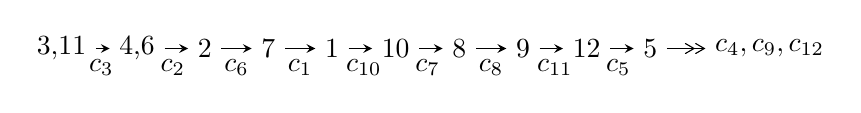
\begin{tikzpicture}[x=23pt, y=7pt]
	% node
	\node (A0) at (-1/8, 0) {3,11};
	\node (A1) at (17/16, 0) {4,6};
	\node (A2) at (17/8, 0) {2};
	\node (A3) at (25/8, 0) {7};
	\node (A4) at (33/8, 0) {1};
	\node (A5) at (41/8, 0) {10};
	\node (A6) at (49/8, 0) {8};
	\node (A7) at (57/8, 0) {9};
	\node (A8) at (65/8, 0) {12};
	\node (A9) at (73/8, 0) {5};
	\node (C1) at (1/2, -1) {$c_{3}$};
	\node (C2) at (13/8, -1) {$c_{2}$};
	\node (C3) at (21/8, -1) {$c_{6}$};
	\node (C4) at (29/8, -1) {$c_{1}$};
	\node (C5) at (37/8, -1) {$c_{10}$};
	\node (C6) at (45/8, -1) {$c_{7}$};
	\node (C7) at (53/8, -1) {$c_{8}$};
	\node (C8) at (61/8, -1) {$c_{11}$};
	\node (C9) at (69/8, -1) {$c_{5}$};
	\node (A10) at (11, 0) {$c_{4},c_{9},c_{12}$};

	% edge
	\draw[->,>=stealth]	
	(A0) edge (A1) (A1) edge (A2) (A2) edge (A3) (A3) edge (A4) (A4) edge (A5) (A5) edge (A6) (A6) edge (A7) (A7) edge (A8) (A8) edge (A9) ;
	\draw[->>,>={angle 60}]	
	(A9) edge (A10);
\end{tikzpicture} \\ 

\end{tabular} \\

\footnotetext{
The image of knot diagram is generated by the software ``\textbf{Draw programme}" developed by Andrew Bartholomew(\url{http://www.layer8.co.uk/maths/draw/index.htm\#Running-draw}), where we modified some parts for our purpose(\url{https://github.com/CATsTAILs/LinksPainter}).
}\phantom \\ \newline 
\centering \textbf{Ideals for irreducible components\footnotemark of $X_{\text{par}}$} 
 
\begin{align*}
I^u_{1}&=\langle 
81175333063282 u^{24}+30690153292943 u^{23}+\cdots+14692178323546426 b-3242513336998852,\\
\phantom{I^u_{1}}&\phantom{= \langle  }-1.32142\times10^{15} u^{24}+2.10121\times10^{15} u^{23}+\cdots+2.93844\times10^{16} a-4.20080\times10^{16},\;u^{25}- u^{24}+\cdots+16 u+4\rangle \\
I^u_{2}&=\langle 
1.78508\times10^{168} u^{59}+1.43280\times10^{169} u^{58}+\cdots+5.04029\times10^{172} b-1.24666\times10^{173},\\
\phantom{I^u_{2}}&\phantom{= \langle  }8.20931\times10^{173} u^{59}+8.68057\times10^{173} u^{58}+\cdots+1.02973\times10^{176} a+5.66958\times10^{176},\\
\phantom{I^u_{2}}&\phantom{= \langle  }u^{60}+u^{59}+\cdots+289 u+227\rangle \\
I^u_{3}&=\langle 
u^5+u^4+3 u^3+2 u^2+b+2 u+1,\;- u^8- u^7-5 u^6-4 u^5-9 u^4-5 u^3-6 u^2+a-2 u,\\
\phantom{I^u_{3}}&\phantom{= \langle  }u^{10}+u^9+6 u^8+5 u^7+13 u^6+9 u^5+12 u^4+7 u^3+4 u^2+2 u+1\rangle \\
I^u_{4}&=\langle 
16776080628176 u^{27}+79179955700749 u^{26}+\cdots+24691129075282 b+255994971816198,\\
\phantom{I^u_{4}}&\phantom{= \langle  }-331954436821981 u^{27}-912855799370818 u^{26}+\cdots+24691129075282 a-1987962528029584,\\
\phantom{I^u_{4}}&\phantom{= \langle  }u^{28}+2 u^{27}+\cdots+8 u+4\rangle \\
\\
\end{align*}
\raggedright * 4 irreducible components of $\dim_{\mathbb{C}}=0$, with total 123 representations.\\
\footnotetext{All coefficients of polynomials are rational numbers. But the coefficients are sometimes approximated in decimal forms when there is not enough margin.}
\newpage
\renewcommand{\arraystretch}{1}
\centering \section*{I. $I^u_{1}= \langle 8.12\times10^{13} u^{24}+3.07\times10^{13} u^{23}+\cdots+1.47\times10^{16} b-3.24\times10^{15},\;-1.32\times10^{15} u^{24}+2.10\times10^{15} u^{23}+\cdots+2.94\times10^{16} a-4.20\times10^{16},\;u^{25}- u^{24}+\cdots+16 u+4 \rangle$}
\flushleft \textbf{(i) Arc colorings}\\
\begin{tabular}{m{7pt} m{180pt} m{7pt} m{180pt} }
\flushright $a_{3}=$&$\begin{pmatrix}1\\0\end{pmatrix}$ \\
\flushright $a_{11}=$&$\begin{pmatrix}0\\u\end{pmatrix}$ \\
\flushright $a_{4}=$&$\begin{pmatrix}1\\u^2\end{pmatrix}$ \\
\flushright $a_{6}=$&$\begin{pmatrix}0.0449701 u^{24}-0.0715078 u^{23}+\cdots-0.542106 u+1.42960\\-0.00552507 u^{24}-0.00208888 u^{23}+\cdots+0.581749 u+0.220697\end{pmatrix}$ \\
\flushright $a_{2}=$&$\begin{pmatrix}0.0263934 u^{24}-0.121687 u^{23}+\cdots+1.62285 u+1.66323\\0.0406210 u^{24}-0.0468137 u^{23}+\cdots+1.43529 u+0.315002\end{pmatrix}$ \\
\flushright $a_{7}=$&$\begin{pmatrix}0.105850 u^{24}-0.0806724 u^{23}+\cdots+2.97593 u+2.35666\\0.0193466 u^{24}-0.0661674 u^{23}+\cdots-0.842412 u-0.0345387\end{pmatrix}$ \\
\flushright $a_{1}=$&$\begin{pmatrix}0.0476780 u^{24}-0.209975 u^{23}+\cdots+1.63902 u+1.59706\\0.0541918 u^{24}+0.0416602 u^{23}+\cdots+2.42220 u+0.583015\end{pmatrix}$ \\
\flushright $a_{10}=$&$\begin{pmatrix}u\\u^3+u\end{pmatrix}$ \\
\flushright $a_{8}=$&$\begin{pmatrix}0.160052 u^{24}-0.146654 u^{23}+\cdots+3.13660 u+2.52396\\0.0265376 u^{24}-0.0541059 u^{23}+\cdots-0.710082 u+0.179880\end{pmatrix}$ \\
\flushright $a_{9}=$&$\begin{pmatrix}0.133514 u^{24}-0.0925477 u^{23}+\cdots+3.84668 u+2.34408\\0.0189237 u^{24}-0.0163606 u^{23}+\cdots-0.400984 u+0.201981\end{pmatrix}$ \\
\flushright $a_{12}=$&$\begin{pmatrix}0.326043 u^{24}-0.239402 u^{23}+\cdots+5.88596 u+2.83366\\-0.0981597 u^{24}+0.00638083 u^{23}+\cdots+0.203450 u+0.196612\end{pmatrix}$ \\
\flushright $a_{5}=$&$\begin{pmatrix}0.0859368 u^{24}-0.160051 u^{23}+\cdots-0.334258 u+0.895546\\-0.00296197 u^{24}+0.00385475 u^{23}+\cdots+0.480951 u+0.145002\end{pmatrix}$\\&\end{tabular}
\flushleft \textbf{(ii) Obstruction class $= -1$}\\~\\
\flushleft \textbf{(iii) Cusp Shapes $= -\frac{2216884505248312}{7346089161773213} u^{24}+\frac{2474930584341802}{7346089161773213} u^{23}+\cdots-\frac{40988520351799862}{7346089161773213} u-\frac{70154967845383976}{7346089161773213}$}\\~\\
\newpage\renewcommand{\arraystretch}{1}
\flushleft \textbf{(iv) u-Polynomials at the component}\newline \\
\begin{tabular}{m{50pt}|m{274pt}}
Crossings & \hspace{64pt}u-Polynomials at each crossing \\
\hline $$\begin{aligned}c_{1},c_{4}\end{aligned}$$&$\begin{aligned}
&u^{25}- u^{24}+\cdots+20 u+1
\end{aligned}$\\
\hline $$\begin{aligned}c_{2},c_{6}\end{aligned}$$&$\begin{aligned}
&u^{25}-8 u^{24}+\cdots-22 u+20
\end{aligned}$\\
\hline $$\begin{aligned}c_{3},c_{5},c_{8}\\c_{10}\end{aligned}$$&$\begin{aligned}
&u^{25}- u^{24}+\cdots+16 u+4
\end{aligned}$\\
\hline $$\begin{aligned}c_{7},c_{9}\end{aligned}$$&$\begin{aligned}
&u^{25}+6 u^{23}+\cdots- u+1
\end{aligned}$\\
\hline $$\begin{aligned}c_{11}\end{aligned}$$&$\begin{aligned}
&u^{25}+17 u^{24}+\cdots+1986 u+292
\end{aligned}$\\
\hline $$\begin{aligned}c_{12}\end{aligned}$$&$\begin{aligned}
&u^{25}+29 u^{24}+\cdots+90112 u+8192
\end{aligned}$\\
\hline
\end{tabular}\\~\\
\newpage\renewcommand{\arraystretch}{1}
\flushleft \textbf{(v) Riley Polynomials at the component}\newline \\
\begin{tabular}{m{50pt}|m{274pt}}
Crossings & \hspace{64pt}Riley Polynomials at each crossing \\
\hline $$\begin{aligned}c_{1},c_{4}\end{aligned}$$&$\begin{aligned}
&y^{25}+37 y^{24}+\cdots+186 y-1
\end{aligned}$\\
\hline $$\begin{aligned}c_{2},c_{6}\end{aligned}$$&$\begin{aligned}
&y^{25}+8 y^{24}+\cdots+1244 y-400
\end{aligned}$\\
\hline $$\begin{aligned}c_{3},c_{5},c_{8}\\c_{10}\end{aligned}$$&$\begin{aligned}
&y^{25}+27 y^{24}+\cdots+80 y-16
\end{aligned}$\\
\hline $$\begin{aligned}c_{7},c_{9}\end{aligned}$$&$\begin{aligned}
&y^{25}+12 y^{24}+\cdots-39 y-1
\end{aligned}$\\
\hline $$\begin{aligned}c_{11}\end{aligned}$$&$\begin{aligned}
&y^{25}- y^{24}+\cdots-613924 y-85264
\end{aligned}$\\
\hline $$\begin{aligned}c_{12}\end{aligned}$$&$\begin{aligned}
&y^{25}-15 y^{24}+\cdots+469762048 y-67108864
\end{aligned}$\\
\hline
\end{tabular}\\~\\
\newpage\flushleft \textbf{(vi) Complex Volumes and Cusp Shapes}
$$\begin{array}{c|c|c}  
\text{Solutions to }I^u_{1}& \I (\text{vol} + \sqrt{-1}CS) & \text{Cusp shape}\\
 \hline 
\begin{aligned}
u &= \phantom{-}0.356781 + 0.935663 I \\
a &= -1.010680 + 0.364892 I \\
b &= -0.135584 + 0.828584 I\end{aligned}
 & \phantom{-}4.71782 - 3.78505 I & -1.08130 + 4.52429 I \\ \hline\begin{aligned}
u &= \phantom{-}0.356781 - 0.935663 I \\
a &= -1.010680 - 0.364892 I \\
b &= -0.135584 - 0.828584 I\end{aligned}
 & \phantom{-}4.71782 + 3.78505 I & -1.08130 - 4.52429 I \\ \hline\begin{aligned}
u &= \phantom{-}0.955649 + 0.143797 I \\
a &= \phantom{-}0.323056 + 0.156868 I \\
b &= -0.840661 + 0.749782 I\end{aligned}
 & \phantom{-}2.79251 - 4.59559 I & -4.91859 + 6.11356 I \\ \hline\begin{aligned}
u &= \phantom{-}0.955649 - 0.143797 I \\
a &= \phantom{-}0.323056 - 0.156868 I \\
b &= -0.840661 - 0.749782 I\end{aligned}
 & \phantom{-}2.79251 + 4.59559 I & -4.91859 - 6.11356 I \\ \hline\begin{aligned}
u &= -0.443877 + 1.205860 I \\
a &= -1.330180 + 0.229600 I \\
b &= \phantom{-}0.418639 + 0.822145 I\end{aligned}
 & \phantom{-}4.34108 + 5.05136 I & -4.70774 - 3.42318 I \\ \hline\begin{aligned}
u &= -0.443877 - 1.205860 I \\
a &= -1.330180 - 0.229600 I \\
b &= \phantom{-}0.418639 - 0.822145 I\end{aligned}
 & \phantom{-}4.34108 - 5.05136 I & -4.70774 + 3.42318 I \\ \hline\begin{aligned}
u &= -0.678966 + 0.135775 I \\
a &= \phantom{-}0.930489 + 0.854461 I \\
b &= -0.673372 + 0.921554 I\end{aligned}
 & \phantom{-}2.14403 - 0.99025 I & -7.34445 - 1.53442 I \\ \hline\begin{aligned}
u &= -0.678966 - 0.135775 I \\
a &= \phantom{-}0.930489 - 0.854461 I \\
b &= -0.673372 - 0.921554 I\end{aligned}
 & \phantom{-}2.14403 + 0.99025 I & -7.34445 + 1.53442 I \\ \hline\begin{aligned}
u &= -0.156784 + 1.353090 I \\
a &= \phantom{-}1.72576 + 0.14878 I \\
b &= -0.90179 - 1.12633 I\end{aligned}
 & \phantom{-}10.67230 + 2.17630 I & \phantom{-}0.04174 + 1.53653 I \\ \hline\begin{aligned}
u &= -0.156784 - 1.353090 I \\
a &= \phantom{-}1.72576 - 0.14878 I \\
b &= -0.90179 + 1.12633 I\end{aligned}
 & \phantom{-}10.67230 - 2.17630 I & \phantom{-}0.04174 - 1.53653 I\\
 \hline 
 \end{array}$$\newpage$$\begin{array}{c|c|c}  
\text{Solutions to }I^u_{1}& \I (\text{vol} + \sqrt{-1}CS) & \text{Cusp shape}\\
 \hline 
\begin{aligned}
u &= \phantom{-}0.367112 + 0.493386 I \\
a &= \phantom{-}2.07051 - 0.52494 I \\
b &= \phantom{-}0.180406 + 1.142870 I\end{aligned}
 & -4.21532 + 1.65565 I & -18.4972 + 2.9896 I \\ \hline\begin{aligned}
u &= \phantom{-}0.367112 - 0.493386 I \\
a &= \phantom{-}2.07051 + 0.52494 I \\
b &= \phantom{-}0.180406 - 1.142870 I\end{aligned}
 & -4.21532 - 1.65565 I & -18.4972 - 2.9896 I \\ \hline\begin{aligned}
u &= -0.03076 + 1.42689 I \\
a &= \phantom{-}1.38281 + 0.68917 I \\
b &= -1.011890 - 0.838182 I\end{aligned}
 & \phantom{-}11.56050 + 4.89672 I & \phantom{-}2.97284 - 7.85735 I \\ \hline\begin{aligned}
u &= -0.03076 - 1.42689 I \\
a &= \phantom{-}1.38281 - 0.68917 I \\
b &= -1.011890 + 0.838182 I\end{aligned}
 & \phantom{-}11.56050 - 4.89672 I & \phantom{-}2.97284 + 7.85735 I \\ \hline\begin{aligned}
u &= -0.03578 + 1.50371 I \\
a &= -0.432938 + 0.103827 I \\
b &= \phantom{-}0.34268 - 1.63762 I\end{aligned}
 & \phantom{-}2.81426 - 3.91771 I & -1.29620 + 2.19890 I \\ \hline\begin{aligned}
u &= -0.03578 - 1.50371 I \\
a &= -0.432938 - 0.103827 I \\
b &= \phantom{-}0.34268 + 1.63762 I\end{aligned}
 & \phantom{-}2.81426 + 3.91771 I & -1.29620 - 2.19890 I \\ \hline\begin{aligned}
u &= -0.319157 + 0.375086 I \\
a &= \phantom{-}0.787826 - 0.669604 I \\
b &= -0.268609 - 0.688871 I\end{aligned}
 & -0.332739 + 1.160480 I & -3.99385 - 5.99928 I \\ \hline\begin{aligned}
u &= -0.319157 - 0.375086 I \\
a &= \phantom{-}0.787826 + 0.669604 I \\
b &= -0.268609 + 0.688871 I\end{aligned}
 & -0.332739 - 1.160480 I & -3.99385 + 5.99928 I \\ \hline\begin{aligned}
u &= \phantom{-}0.47309 + 1.48937 I \\
a &= -1.051700 - 0.257525 I \\
b &= \phantom{-}1.116970 - 0.232182 I\end{aligned}
 & \phantom{-}7.93268 - 2.23602 I & \phantom{-}0.761695 + 0.334356 I \\ \hline\begin{aligned}
u &= \phantom{-}0.47309 - 1.48937 I \\
a &= -1.051700 + 0.257525 I \\
b &= \phantom{-}1.116970 + 0.232182 I\end{aligned}
 & \phantom{-}7.93268 + 2.23602 I & \phantom{-}0.761695 - 0.334356 I\\
 \hline 
 \end{array}$$\newpage$$\begin{array}{c|c|c}  
\text{Solutions to }I^u_{1}& \I (\text{vol} + \sqrt{-1}CS) & \text{Cusp shape}\\
 \hline 
\begin{aligned}
u &= -0.332884\phantom{ +0.000000I} \\
a &= \phantom{-}1.83055\phantom{ +0.000000I} \\
b &= \phantom{-}0.306235\phantom{ +0.000000I}\end{aligned}
 & -1.10902\phantom{ +0.000000I} & -7.26140\phantom{ +0.000000I} \\ \hline\begin{aligned}
u &= \phantom{-}0.62513 + 1.55416 I \\
a &= \phantom{-}1.381370 + 0.302300 I \\
b &= -1.00799 + 1.26430 I\end{aligned}
 & \phantom{-}13.3035 - 17.0719 I & -2.40849 + 7.81401 I \\ \hline\begin{aligned}
u &= \phantom{-}0.62513 - 1.55416 I \\
a &= \phantom{-}1.381370 - 0.302300 I \\
b &= -1.00799 - 1.26430 I\end{aligned}
 & \phantom{-}13.3035 + 17.0719 I & -2.40849 - 7.81401 I \\ \hline\begin{aligned}
u &= -0.44600 + 1.67824 I \\
a &= \phantom{-}0.808407 - 0.509554 I \\
b &= -1.37193 + 0.86362 I\end{aligned}
 & \phantom{-}14.7335 + 8.6358 I & -0.89771 - 3.83191 I \\ \hline\begin{aligned}
u &= -0.44600 - 1.67824 I \\
a &= \phantom{-}0.808407 + 0.509554 I \\
b &= -1.37193 - 0.86362 I\end{aligned}
 & \phantom{-}14.7335 - 8.6358 I & -0.89771 + 3.83191 I\\
 \hline 
 \end{array}$$\newpage\newpage\renewcommand{\arraystretch}{1}
\centering \section*{II. $I^u_{2}= \langle 1.79\times10^{168} u^{59}+1.43\times10^{169} u^{58}+\cdots+5.04\times10^{172} b-1.25\times10^{173},\;8.21\times10^{173} u^{59}+8.68\times10^{173} u^{58}+\cdots+1.03\times10^{176} a+5.67\times10^{176},\;u^{60}+u^{59}+\cdots+289 u+227 \rangle$}
\flushleft \textbf{(i) Arc colorings}\\
\begin{tabular}{m{7pt} m{180pt} m{7pt} m{180pt} }
\flushright $a_{3}=$&$\begin{pmatrix}1\\0\end{pmatrix}$ \\
\flushright $a_{11}=$&$\begin{pmatrix}0\\u\end{pmatrix}$ \\
\flushright $a_{4}=$&$\begin{pmatrix}1\\u^2\end{pmatrix}$ \\
\flushright $a_{6}=$&$\begin{pmatrix}-0.00797228 u^{59}-0.00842993 u^{58}+\cdots+9.12745 u-5.50588\\-0.0000354162 u^{59}-0.000284270 u^{58}+\cdots-4.15178 u+2.47338\end{pmatrix}$ \\
\flushright $a_{2}=$&$\begin{pmatrix}0.00875654 u^{59}+0.00749914 u^{58}+\cdots+11.5546 u+7.51424\\-0.00793371 u^{59}-0.00743256 u^{58}+\cdots-8.38811 u-1.46531\end{pmatrix}$ \\
\flushright $a_{7}=$&$\begin{pmatrix}-0.0162583 u^{59}-0.0123765 u^{58}+\cdots-26.6169 u+2.33453\\-0.00855045 u^{59}-0.00916146 u^{58}+\cdots+0.843688 u-4.75348\end{pmatrix}$ \\
\flushright $a_{1}=$&$\begin{pmatrix}0.00262878 u^{59}+0.00246517 u^{58}+\cdots+4.79084 u+5.76350\\-0.00901992 u^{59}-0.00861896 u^{58}+\cdots-7.31321 u-1.71360\end{pmatrix}$ \\
\flushright $a_{10}=$&$\begin{pmatrix}u\\u^3+u\end{pmatrix}$ \\
\flushright $a_{8}=$&$\begin{pmatrix}-0.0188007 u^{59}-0.0151359 u^{58}+\cdots-25.8727 u+1.23865\\-0.00969922 u^{59}-0.0110547 u^{58}+\cdots+2.22778 u-5.80010\end{pmatrix}$ \\
\flushright $a_{9}=$&$\begin{pmatrix}-0.0117646 u^{59}-0.0129427 u^{58}+\cdots-2.49013 u-2.12575\\-0.0129451 u^{59}-0.0143337 u^{58}+\cdots-2.64558 u-7.90726\end{pmatrix}$ \\
\flushright $a_{12}=$&$\begin{pmatrix}0.0212826 u^{59}+0.0118027 u^{58}+\cdots+59.9419 u-6.26228\\0.00838830 u^{59}+0.00778421 u^{58}+\cdots+18.9048 u+5.25987\end{pmatrix}$ \\
\flushright $a_{5}=$&$\begin{pmatrix}0.00318861 u^{59}-0.00358656 u^{58}+\cdots+16.6160 u-18.5879\\0.0112699 u^{59}+0.00793128 u^{58}+\cdots+14.3076 u-7.16173\end{pmatrix}$\\&\end{tabular}
\flushleft \textbf{(ii) Obstruction class $= -1$}\\~\\
\flushleft \textbf{(iii) Cusp Shapes $= 0.00763493 u^{59}+0.0171335 u^{58}+\cdots-50.7125 u+29.2529$}\\~\\
\newpage\renewcommand{\arraystretch}{1}
\flushleft \textbf{(iv) u-Polynomials at the component}\newline \\
\begin{tabular}{m{50pt}|m{274pt}}
Crossings & \hspace{64pt}u-Polynomials at each crossing \\
\hline $$\begin{aligned}c_{1},c_{4}\end{aligned}$$&$\begin{aligned}
&u^{60}-5 u^{59}+\cdots-61367 u+12433
\end{aligned}$\\
\hline $$\begin{aligned}c_{2},c_{6}\end{aligned}$$&$\begin{aligned}
&(u^{30}+3 u^{29}+\cdots+3 u+1)^{2}
\end{aligned}$\\
\hline $$\begin{aligned}c_{3},c_{5},c_{8}\\c_{10}\end{aligned}$$&$\begin{aligned}
&u^{60}+u^{59}+\cdots+289 u+227
\end{aligned}$\\
\hline $$\begin{aligned}c_{7},c_{9}\end{aligned}$$&$\begin{aligned}
&u^{60}-3 u^{59}+\cdots-8079 u+2305
\end{aligned}$\\
\hline $$\begin{aligned}c_{11}\end{aligned}$$&$\begin{aligned}
&(u^{30}-7 u^{29}+\cdots+726 u-59)^{2}
\end{aligned}$\\
\hline $$\begin{aligned}c_{12}\end{aligned}$$&$\begin{aligned}
&(u^{30}-10 u^{29}+\cdots-2853 u-591)^{2}
\end{aligned}$\\
\hline
\end{tabular}\\~\\
\newpage\renewcommand{\arraystretch}{1}
\flushleft \textbf{(v) Riley Polynomials at the component}\newline \\
\begin{tabular}{m{50pt}|m{274pt}}
Crossings & \hspace{64pt}Riley Polynomials at each crossing \\
\hline $$\begin{aligned}c_{1},c_{4}\end{aligned}$$&$\begin{aligned}
&y^{60}+51 y^{59}+\cdots-2575299743 y+154579489
\end{aligned}$\\
\hline $$\begin{aligned}c_{2},c_{6}\end{aligned}$$&$\begin{aligned}
&(y^{30}+9 y^{29}+\cdots-3 y+1)^{2}
\end{aligned}$\\
\hline $$\begin{aligned}c_{3},c_{5},c_{8}\\c_{10}\end{aligned}$$&$\begin{aligned}
&y^{60}+41 y^{59}+\cdots+250623 y+51529
\end{aligned}$\\
\hline $$\begin{aligned}c_{7},c_{9}\end{aligned}$$&$\begin{aligned}
&y^{60}+5 y^{59}+\cdots+133586719 y+5313025
\end{aligned}$\\
\hline $$\begin{aligned}c_{11}\end{aligned}$$&$\begin{aligned}
&(y^{30}+17 y^{29}+\cdots-464182 y+3481)^{2}
\end{aligned}$\\
\hline $$\begin{aligned}c_{12}\end{aligned}$$&$\begin{aligned}
&(y^{30}-30 y^{29}+\cdots-17977395 y+349281)^{2}
\end{aligned}$\\
\hline
\end{tabular}\\~\\
\newpage\flushleft \textbf{(vi) Complex Volumes and Cusp Shapes}
$$\begin{array}{c|c|c}  
\text{Solutions to }I^u_{2}& \I (\text{vol} + \sqrt{-1}CS) & \text{Cusp shape}\\
 \hline 
\begin{aligned}
u &= -0.151089 + 0.988984 I \\
a &= \phantom{-}1.015950 - 0.753380 I \\
b &= -0.268673 - 0.905256 I\end{aligned}
 & \phantom{-}0.331844 + 0.773996 I & -5.81323 - 0.94934 I \\ \hline\begin{aligned}
u &= -0.151089 - 0.988984 I \\
a &= \phantom{-}1.015950 + 0.753380 I \\
b &= -0.268673 + 0.905256 I\end{aligned}
 & \phantom{-}0.331844 - 0.773996 I & -5.81323 + 0.94934 I \\ \hline\begin{aligned}
u &= -0.197498 + 0.949193 I \\
a &= \phantom{-}0.054102 - 0.941860 I \\
b &= -0.09788 + 1.49969 I\end{aligned}
 & -6.07488 + 0.77241 I & -12.7372 - 14.9639 I \\ \hline\begin{aligned}
u &= -0.197498 - 0.949193 I \\
a &= \phantom{-}0.054102 + 0.941860 I \\
b &= -0.09788 - 1.49969 I\end{aligned}
 & -6.07488 - 0.77241 I & -12.7372 + 14.9639 I \\ \hline\begin{aligned}
u &= \phantom{-}0.326973 + 0.865535 I \\
a &= \phantom{-}1.17062 + 1.94335 I \\
b &= -0.220348 + 0.210562 I\end{aligned}
 & -1.05655 - 1.42739 I & \phantom{-}10.99269 - 2.14037 I \\ \hline\begin{aligned}
u &= \phantom{-}0.326973 - 0.865535 I \\
a &= \phantom{-}1.17062 - 1.94335 I \\
b &= -0.220348 - 0.210562 I\end{aligned}
 & -1.05655 + 1.42739 I & \phantom{-}10.99269 + 2.14037 I \\ \hline\begin{aligned}
u &= \phantom{-}0.599443 + 0.897678 I \\
a &= \phantom{-}0.310619 - 0.931457 I \\
b &= \phantom{-}0.476833\phantom{ +0.000000I}\end{aligned}
 & \phantom{-}5.08000\phantom{ +0.000000I} & \phantom{-0.000000 } 0 \\ \hline\begin{aligned}
u &= \phantom{-}0.599443 - 0.897678 I \\
a &= \phantom{-}0.310619 + 0.931457 I \\
b &= \phantom{-}0.476833\phantom{ +0.000000I}\end{aligned}
 & \phantom{-}5.08000\phantom{ +0.000000I} & \phantom{-0.000000 } 0 \\ \hline\begin{aligned}
u &= \phantom{-}0.843197 + 0.154861 I \\
a &= \phantom{-}0.154657 - 0.463896 I \\
b &= -0.824890 - 0.215589 I\end{aligned}
 & \phantom{-}3.05304 + 2.77277 I & -2.69988 - 3.50142 I \\ \hline\begin{aligned}
u &= \phantom{-}0.843197 - 0.154861 I \\
a &= \phantom{-}0.154657 + 0.463896 I \\
b &= -0.824890 + 0.215589 I\end{aligned}
 & \phantom{-}3.05304 - 2.77277 I & -2.69988 + 3.50142 I\\
 \hline 
 \end{array}$$\newpage$$\begin{array}{c|c|c}  
\text{Solutions to }I^u_{2}& \I (\text{vol} + \sqrt{-1}CS) & \text{Cusp shape}\\
 \hline 
\begin{aligned}
u &= -0.830816 + 0.161998 I \\
a &= \phantom{-}0.563539 - 0.534434 I \\
b &= -0.268673 - 0.905256 I\end{aligned}
 & \phantom{-}0.331844 + 0.773996 I & -5.81323 - 0.94934 I \\ \hline\begin{aligned}
u &= -0.830816 - 0.161998 I \\
a &= \phantom{-}0.563539 + 0.534434 I \\
b &= -0.268673 + 0.905256 I\end{aligned}
 & \phantom{-}0.331844 - 0.773996 I & -5.81323 + 0.94934 I \\ \hline\begin{aligned}
u &= \phantom{-}0.007925 + 0.844615 I \\
a &= -1.81193 - 2.76865 I \\
b &= \phantom{-}0.258541 + 0.333070 I\end{aligned}
 & \phantom{-}1.89101 + 5.03315 I & \phantom{-}1.75905 - 6.82138 I \\ \hline\begin{aligned}
u &= \phantom{-}0.007925 - 0.844615 I \\
a &= -1.81193 + 2.76865 I \\
b &= \phantom{-}0.258541 - 0.333070 I\end{aligned}
 & \phantom{-}1.89101 - 5.03315 I & \phantom{-}1.75905 + 6.82138 I \\ \hline\begin{aligned}
u &= \phantom{-}0.477112 + 1.090850 I \\
a &= -1.06340 - 1.18158 I \\
b &= \phantom{-}0.677641 - 0.588433 I\end{aligned}
 & \phantom{-}5.72749 - 7.45875 I & \phantom{-0.000000 } 0 \\ \hline\begin{aligned}
u &= \phantom{-}0.477112 - 1.090850 I \\
a &= -1.06340 + 1.18158 I \\
b &= \phantom{-}0.677641 + 0.588433 I\end{aligned}
 & \phantom{-}5.72749 + 7.45875 I & \phantom{-0.000000 } 0 \\ \hline\begin{aligned}
u &= \phantom{-}0.433233 + 1.120270 I \\
a &= \phantom{-}0.645877 + 0.522724 I \\
b &= -0.106768 + 1.224240 I\end{aligned}
 & -2.00126 - 5.14743 I & \phantom{-0.000000 } 0 \\ \hline\begin{aligned}
u &= \phantom{-}0.433233 - 1.120270 I \\
a &= \phantom{-}0.645877 - 0.522724 I \\
b &= -0.106768 - 1.224240 I\end{aligned}
 & -2.00126 + 5.14743 I & \phantom{-0.000000 } 0 \\ \hline\begin{aligned}
u &= -0.464555 + 1.178190 I \\
a &= \phantom{-}0.234302 + 0.213986 I \\
b &= \phantom{-}0.097409 - 1.142310 I\end{aligned}
 & \phantom{-}3.33083 + 3.97209 I & \phantom{-0.000000 } 0 \\ \hline\begin{aligned}
u &= -0.464555 - 1.178190 I \\
a &= \phantom{-}0.234302 - 0.213986 I \\
b &= \phantom{-}0.097409 + 1.142310 I\end{aligned}
 & \phantom{-}3.33083 - 3.97209 I & \phantom{-0.000000 } 0\\
 \hline 
 \end{array}$$\newpage$$\begin{array}{c|c|c}  
\text{Solutions to }I^u_{2}& \I (\text{vol} + \sqrt{-1}CS) & \text{Cusp shape}\\
 \hline 
\begin{aligned}
u &= -0.385734 + 0.615064 I \\
a &= -0.13976 + 1.50771 I \\
b &= \phantom{-}0.556018\phantom{ +0.000000I}\end{aligned}
 & -0.861477\phantom{ +0.000000I} & -2.21853 + 0. I\phantom{ +0.000000I} \\ \hline\begin{aligned}
u &= -0.385734 - 0.615064 I \\
a &= -0.13976 - 1.50771 I \\
b &= \phantom{-}0.556018\phantom{ +0.000000I}\end{aligned}
 & -0.861477\phantom{ +0.000000I} & -2.21853 + 0. I\phantom{ +0.000000I} \\ \hline\begin{aligned}
u &= -0.191587 + 1.292350 I \\
a &= -0.735001 + 0.950554 I \\
b &= \phantom{-}0.097409 + 1.142310 I\end{aligned}
 & \phantom{-}3.33083 - 3.97209 I & \phantom{-0.000000 } 0 \\ \hline\begin{aligned}
u &= -0.191587 - 1.292350 I \\
a &= -0.735001 - 0.950554 I \\
b &= \phantom{-}0.097409 - 1.142310 I\end{aligned}
 & \phantom{-}3.33083 + 3.97209 I & \phantom{-0.000000 } 0 \\ \hline\begin{aligned}
u &= -0.720332 + 1.143500 I \\
a &= -0.265603 + 0.406457 I \\
b &= \phantom{-}0.258541 + 0.333070 I\end{aligned}
 & \phantom{-}1.89101 + 5.03315 I & \phantom{-0.000000 } 0 \\ \hline\begin{aligned}
u &= -0.720332 - 1.143500 I \\
a &= -0.265603 - 0.406457 I \\
b &= \phantom{-}0.258541 - 0.333070 I\end{aligned}
 & \phantom{-}1.89101 - 5.03315 I & \phantom{-0.000000 } 0 \\ \hline\begin{aligned}
u &= -1.334490 + 0.240948 I \\
a &= \phantom{-}0.168255 + 0.261950 I \\
b &= -0.220348 - 0.210562 I\end{aligned}
 & -1.05655 + 1.42739 I & \phantom{-0.000000 } 0 \\ \hline\begin{aligned}
u &= -1.334490 - 0.240948 I \\
a &= \phantom{-}0.168255 - 0.261950 I \\
b &= -0.220348 + 0.210562 I\end{aligned}
 & -1.05655 - 1.42739 I & \phantom{-0.000000 } 0 \\ \hline\begin{aligned}
u &= \phantom{-}0.167787 + 1.359600 I \\
a &= -1.33826 - 0.70122 I \\
b &= \phantom{-}0.810607 + 0.866117 I\end{aligned}
 & \phantom{-}6.78367 + 0.73525 I & \phantom{-0.000000 } 0 \\ \hline\begin{aligned}
u &= \phantom{-}0.167787 - 1.359600 I \\
a &= -1.33826 + 0.70122 I \\
b &= \phantom{-}0.810607 - 0.866117 I\end{aligned}
 & \phantom{-}6.78367 - 0.73525 I & \phantom{-0.000000 } 0\\
 \hline 
 \end{array}$$\newpage$$\begin{array}{c|c|c}  
\text{Solutions to }I^u_{2}& \I (\text{vol} + \sqrt{-1}CS) & \text{Cusp shape}\\
 \hline 
\begin{aligned}
u &= -0.115657 + 1.370730 I \\
a &= \phantom{-}0.911391 + 0.108509 I \\
b &= -0.824890 - 0.215589 I\end{aligned}
 & \phantom{-}3.05304 + 2.77277 I & \phantom{-0.000000 } 0 \\ \hline\begin{aligned}
u &= -0.115657 - 1.370730 I \\
a &= \phantom{-}0.911391 - 0.108509 I \\
b &= -0.824890 + 0.215589 I\end{aligned}
 & \phantom{-}3.05304 - 2.77277 I & \phantom{-0.000000 } 0 \\ \hline\begin{aligned}
u &= \phantom{-}0.19606 + 1.42365 I \\
a &= \phantom{-}1.44865 - 0.22898 I \\
b &= -1.04755 + 1.32743 I\end{aligned}
 & \phantom{-}11.53870 - 7.55219 I & \phantom{-0.000000 } 0 \\ \hline\begin{aligned}
u &= \phantom{-}0.19606 - 1.42365 I \\
a &= \phantom{-}1.44865 + 0.22898 I \\
b &= -1.04755 - 1.32743 I\end{aligned}
 & \phantom{-}11.53870 + 7.55219 I & \phantom{-0.000000 } 0 \\ \hline\begin{aligned}
u &= -0.13751 + 1.44639 I \\
a &= -1.139830 + 0.571849 I \\
b &= \phantom{-}1.11980 - 1.17245 I\end{aligned}
 & \phantom{-}7.57073 + 1.54799 I & \phantom{-0.000000 } 0 \\ \hline\begin{aligned}
u &= -0.13751 - 1.44639 I \\
a &= -1.139830 - 0.571849 I \\
b &= \phantom{-}1.11980 + 1.17245 I\end{aligned}
 & \phantom{-}7.57073 - 1.54799 I & \phantom{-0.000000 } 0 \\ \hline\begin{aligned}
u &= -0.39296 + 1.43423 I \\
a &= -1.60846 - 0.05755 I \\
b &= \phantom{-}0.836436 + 0.962571 I\end{aligned}
 & \phantom{-}6.51793 + 5.45084 I & \phantom{-0.000000 } 0 \\ \hline\begin{aligned}
u &= -0.39296 - 1.43423 I \\
a &= -1.60846 + 0.05755 I \\
b &= \phantom{-}0.836436 - 0.962571 I\end{aligned}
 & \phantom{-}6.51793 - 5.45084 I & \phantom{-0.000000 } 0 \\ \hline\begin{aligned}
u &= \phantom{-}1.48914 + 0.10011 I \\
a &= \phantom{-}0.22281 + 1.55793 I \\
b &= -0.09788 + 1.49969 I\end{aligned}
 & -6.07488 + 0.77241 I & \phantom{-0.000000 } 0 \\ \hline\begin{aligned}
u &= \phantom{-}1.48914 - 0.10011 I \\
a &= \phantom{-}0.22281 - 1.55793 I \\
b &= -0.09788 - 1.49969 I\end{aligned}
 & -6.07488 - 0.77241 I & \phantom{-0.000000 } 0\\
 \hline 
 \end{array}$$\newpage$$\begin{array}{c|c|c}  
\text{Solutions to }I^u_{2}& \I (\text{vol} + \sqrt{-1}CS) & \text{Cusp shape}\\
 \hline 
\begin{aligned}
u &= \phantom{-}0.08468 + 1.49584 I \\
a &= \phantom{-}1.349320 - 0.340698 I \\
b &= -1.36115 + 0.81924 I\end{aligned}
 & \phantom{-}13.16510 - 1.04438 I & \phantom{-0.000000 } 0 \\ \hline\begin{aligned}
u &= \phantom{-}0.08468 - 1.49584 I \\
a &= \phantom{-}1.349320 + 0.340698 I \\
b &= -1.36115 - 0.81924 I\end{aligned}
 & \phantom{-}13.16510 + 1.04438 I & \phantom{-0.000000 } 0 \\ \hline\begin{aligned}
u &= \phantom{-}0.42436 + 1.45884 I \\
a &= -1.51602 - 0.04319 I \\
b &= \phantom{-}1.11039 - 1.00742 I\end{aligned}
 & \phantom{-}7.97566 - 9.65899 I & \phantom{-0.000000 } 0 \\ \hline\begin{aligned}
u &= \phantom{-}0.42436 - 1.45884 I \\
a &= -1.51602 + 0.04319 I \\
b &= \phantom{-}1.11039 + 1.00742 I\end{aligned}
 & \phantom{-}7.97566 + 9.65899 I & \phantom{-0.000000 } 0 \\ \hline\begin{aligned}
u &= \phantom{-}1.53765 + 0.12330 I \\
a &= -0.300107 - 0.447420 I \\
b &= \phantom{-}1.11039 - 1.00742 I\end{aligned}
 & \phantom{-}7.97566 - 9.65899 I & \phantom{-0.000000 } 0 \\ \hline\begin{aligned}
u &= \phantom{-}1.53765 - 0.12330 I \\
a &= -0.300107 + 0.447420 I \\
b &= \phantom{-}1.11039 + 1.00742 I\end{aligned}
 & \phantom{-}7.97566 + 9.65899 I & \phantom{-0.000000 } 0 \\ \hline\begin{aligned}
u &= -0.33599 + 1.58079 I \\
a &= -1.043490 - 0.349969 I \\
b &= \phantom{-}0.677641 + 0.588433 I\end{aligned}
 & \phantom{-}5.72749 + 7.45875 I & \phantom{-0.000000 } 0 \\ \hline\begin{aligned}
u &= -0.33599 - 1.58079 I \\
a &= -1.043490 + 0.349969 I \\
b &= \phantom{-}0.677641 - 0.588433 I\end{aligned}
 & \phantom{-}5.72749 - 7.45875 I & \phantom{-0.000000 } 0 \\ \hline\begin{aligned}
u &= -1.61765 + 0.46633 I \\
a &= -0.174220 - 0.449001 I \\
b &= \phantom{-}1.11980 - 1.17245 I\end{aligned}
 & \phantom{-}7.57073 + 1.54799 I & \phantom{-0.000000 } 0 \\ \hline\begin{aligned}
u &= -1.61765 - 0.46633 I \\
a &= -0.174220 + 0.449001 I \\
b &= \phantom{-}1.11980 + 1.17245 I\end{aligned}
 & \phantom{-}7.57073 - 1.54799 I & \phantom{-0.000000 } 0\\
 \hline 
 \end{array}$$\newpage$$\begin{array}{c|c|c}  
\text{Solutions to }I^u_{2}& \I (\text{vol} + \sqrt{-1}CS) & \text{Cusp shape}\\
 \hline 
\begin{aligned}
u &= -0.199803 + 0.244970 I \\
a &= \phantom{-}4.38347 + 3.03006 I \\
b &= -0.106768 - 1.224240 I\end{aligned}
 & -2.00126 + 5.14743 I & -12.34153 - 6.38581 I \\ \hline\begin{aligned}
u &= -0.199803 - 0.244970 I \\
a &= \phantom{-}4.38347 - 3.03006 I \\
b &= -0.106768 + 1.224240 I\end{aligned}
 & -2.00126 - 5.14743 I & -12.34153 + 6.38581 I \\ \hline\begin{aligned}
u &= -0.154498 + 0.258494 I \\
a &= \phantom{-}1.97537 - 0.70610 I \\
b &= \phantom{-}0.810607 - 0.866117 I\end{aligned}
 & \phantom{-}6.78367 - 0.73525 I & \phantom{-}1.34056 + 4.28994 I \\ \hline\begin{aligned}
u &= -0.154498 - 0.258494 I \\
a &= \phantom{-}1.97537 + 0.70610 I \\
b &= \phantom{-}0.810607 + 0.866117 I\end{aligned}
 & \phantom{-}6.78367 + 0.73525 I & \phantom{-}1.34056 - 4.28994 I \\ \hline\begin{aligned}
u &= \phantom{-}0.283976 + 0.026888 I \\
a &= \phantom{-}1.65738 - 0.91773 I \\
b &= \phantom{-}0.836436 - 0.962571 I\end{aligned}
 & \phantom{-}6.51793 - 5.45084 I & -3.44913 - 0.50892 I \\ \hline\begin{aligned}
u &= \phantom{-}0.283976 - 0.026888 I \\
a &= \phantom{-}1.65738 + 0.91773 I \\
b &= \phantom{-}0.836436 + 0.962571 I\end{aligned}
 & \phantom{-}6.51793 + 5.45084 I & -3.44913 + 0.50892 I \\ \hline\begin{aligned}
u &= -0.81940 + 1.65329 I \\
a &= \phantom{-}1.140340 - 0.437941 I \\
b &= -1.04755 - 1.32743 I\end{aligned}
 & \phantom{-}11.53870 + 7.55219 I & \phantom{-0.000000 } 0 \\ \hline\begin{aligned}
u &= -0.81940 - 1.65329 I \\
a &= \phantom{-}1.140340 + 0.437941 I \\
b &= -1.04755 + 1.32743 I\end{aligned}
 & \phantom{-}11.53870 - 7.55219 I & \phantom{-0.000000 } 0 \\ \hline\begin{aligned}
u &= \phantom{-}0.67804 + 1.80475 I \\
a &= \phantom{-}0.603871 + 0.402297 I \\
b &= -1.36115 - 0.81924 I\end{aligned}
 & \phantom{-}13.16510 + 1.04438 I & \phantom{-0.000000 } 0 \\ \hline\begin{aligned}
u &= \phantom{-}0.67804 - 1.80475 I \\
a &= \phantom{-}0.603871 - 0.402297 I \\
b &= -1.36115 + 0.81924 I\end{aligned}
 & \phantom{-}13.16510 - 1.04438 I & \phantom{-0.000000 } 0\\
 \hline 
 \end{array}$$\newpage\newpage\renewcommand{\arraystretch}{1}
\centering \section*{III. $I^u_{3}= \langle u^5+u^4+3 u^3+2 u^2+b+2 u+1,\;- u^8- u^7+\cdots+a-2 u,\;u^{10}+u^9+\cdots+2 u+1 \rangle$}
\flushleft \textbf{(i) Arc colorings}\\
\begin{tabular}{m{7pt} m{180pt} m{7pt} m{180pt} }
\flushright $a_{3}=$&$\begin{pmatrix}1\\0\end{pmatrix}$ \\
\flushright $a_{11}=$&$\begin{pmatrix}0\\u\end{pmatrix}$ \\
\flushright $a_{4}=$&$\begin{pmatrix}1\\u^2\end{pmatrix}$ \\
\flushright $a_{6}=$&$\begin{pmatrix}u^8+u^7+5 u^6+4 u^5+9 u^4+5 u^3+6 u^2+2 u\\- u^5- u^4-3 u^3-2 u^2-2 u-1\end{pmatrix}$ \\
\flushright $a_{2}=$&$\begin{pmatrix}- u^9- u^8-5 u^7-4 u^6-8 u^5-5 u^4-3 u^3- u^2+2 u+2\\u^9+u^8+5 u^7+4 u^6+9 u^5+6 u^4+7 u^3+4 u^2+2 u\end{pmatrix}$ \\
\flushright $a_{7}=$&$\begin{pmatrix}- u^7- u^6-5 u^5-4 u^4-9 u^3-5 u^2-5 u-2\\- u^9- u^8-5 u^7-4 u^6-9 u^5-5 u^4-6 u^3-2 u^2- u\end{pmatrix}$ \\
\flushright $a_{1}=$&$\begin{pmatrix}- u^9- u^8-5 u^7-4 u^6-8 u^5-5 u^4-2 u^3- u^2+3 u+2\\u^9+u^8+5 u^7+4 u^6+10 u^5+6 u^4+8 u^3+4 u^2+2 u\end{pmatrix}$ \\
\flushright $a_{10}=$&$\begin{pmatrix}u\\u^3+u\end{pmatrix}$ \\
\flushright $a_{8}=$&$\begin{pmatrix}- u^9- u^8-6 u^7-5 u^6-13 u^5-9 u^4-13 u^3-7 u^2-5 u-2\\- u^9- u^8-5 u^7-4 u^6-9 u^5-5 u^4-6 u^3-2 u^2\end{pmatrix}$ \\
\flushright $a_{9}=$&$\begin{pmatrix}- u^7- u^6-4 u^5-4 u^4-7 u^3-5 u^2-5 u-2\\- u^9- u^8-5 u^7-5 u^6-10 u^5-8 u^4-8 u^3-4 u^2- u\end{pmatrix}$ \\
\flushright $a_{12}=$&$\begin{pmatrix}u^9+u^8+5 u^7+5 u^6+11 u^5+9 u^4+13 u^3+7 u^2+6 u+2\\u^8+2 u^7+4 u^6+7 u^5+5 u^4+7 u^3+2 u^2+u\end{pmatrix}$ \\
\flushright $a_{5}=$&$\begin{pmatrix}u^6+2 u^4+u^2\\u^8+3 u^6+3 u^4+u^2\end{pmatrix}$\\&\end{tabular}
\flushleft \textbf{(ii) Obstruction class $= 1$}\\~\\
\flushleft \textbf{(iii) Cusp Shapes $= -5 u^9- u^8-28 u^7-9 u^6-59 u^5-26 u^4-53 u^3-27 u^2-13 u-11$}\\~\\
\newpage\renewcommand{\arraystretch}{1}
\flushleft \textbf{(iv) u-Polynomials at the component}\newline \\
\begin{tabular}{m{50pt}|m{274pt}}
Crossings & \hspace{64pt}u-Polynomials at each crossing \\
\hline $$\begin{aligned}c_{1},c_{4}\end{aligned}$$&$\begin{aligned}
&u^{10}+u^9+2 u^8+u^7-5 u^6+6 u^5+5 u^4-7 u^3+6 u^2-2 u+1
\end{aligned}$\\
\hline $$\begin{aligned}c_{2}\end{aligned}$$&$\begin{aligned}
&u^{10}+3 u^9+8 u^8+13 u^7+19 u^6+18 u^5+17 u^4+9 u^3+6 u^2+2 u+1
\end{aligned}$\\
\hline $$\begin{aligned}c_{3},c_{8}\end{aligned}$$&$\begin{aligned}
&u^{10}+u^9+6 u^8+5 u^7+13 u^6+9 u^5+12 u^4+7 u^3+4 u^2+2 u+1
\end{aligned}$\\
\hline $$\begin{aligned}c_{5},c_{10}\end{aligned}$$&$\begin{aligned}
&u^{10}- u^9+6 u^8-5 u^7+13 u^6-9 u^5+12 u^4-7 u^3+4 u^2-2 u+1
\end{aligned}$\\
\hline $$\begin{aligned}c_{6}\end{aligned}$$&$\begin{aligned}
&u^{10}-3 u^9+8 u^8-13 u^7+19 u^6-18 u^5+17 u^4-9 u^3+6 u^2-2 u+1
\end{aligned}$\\
\hline $$\begin{aligned}c_{7},c_{9}\end{aligned}$$&$\begin{aligned}
&u^{10}-2 u^8-2 u^7+3 u^6+4 u^5-3 u^3-2 u^2+u+1
\end{aligned}$\\
\hline $$\begin{aligned}c_{11}\end{aligned}$$&$\begin{aligned}
&u^{10}+4 u^9+\cdots+200 u+59
\end{aligned}$\\
\hline $$\begin{aligned}c_{12}\end{aligned}$$&$\begin{aligned}
&u^{10}-6 u^8-10 u^7+13 u^6+23 u^5+55 u^4+58 u^3+32 u^2+9 u+1
\end{aligned}$\\
\hline
\end{tabular}\\~\\
\newpage\renewcommand{\arraystretch}{1}
\flushleft \textbf{(v) Riley Polynomials at the component}\newline \\
\begin{tabular}{m{50pt}|m{274pt}}
Crossings & \hspace{64pt}Riley Polynomials at each crossing \\
\hline $$\begin{aligned}c_{1},c_{4}\end{aligned}$$&$\begin{aligned}
&y^{10}+3 y^9-8 y^8-23 y^7+59 y^6-42 y^5+57 y^4+25 y^3+18 y^2+8 y+1
\end{aligned}$\\
\hline $$\begin{aligned}c_{2},c_{6}\end{aligned}$$&$\begin{aligned}
&y^{10}+7 y^9+\cdots+8 y+1
\end{aligned}$\\
\hline $$\begin{aligned}c_{3},c_{5},c_{8}\\c_{10}\end{aligned}$$&$\begin{aligned}
&y^{10}+11 y^9+\cdots+4 y+1
\end{aligned}$\\
\hline $$\begin{aligned}c_{7},c_{9}\end{aligned}$$&$\begin{aligned}
&y^{10}-4 y^9+\cdots-5 y+1
\end{aligned}$\\
\hline $$\begin{aligned}c_{11}\end{aligned}$$&$\begin{aligned}
&y^{10}-4 y^9+\cdots-5898 y+3481
\end{aligned}$\\
\hline $$\begin{aligned}c_{12}\end{aligned}$$&$\begin{aligned}
&y^{10}-12 y^9+\cdots-17 y+1
\end{aligned}$\\
\hline
\end{tabular}\\~\\
\newpage\flushleft \textbf{(vi) Complex Volumes and Cusp Shapes}
$$\begin{array}{c|c|c}  
\text{Solutions to }I^u_{3}& \I (\text{vol} + \sqrt{-1}CS) & \text{Cusp shape}\\
 \hline 
\begin{aligned}
u &= \phantom{-}0.218748 + 1.275640 I \\
a &= -0.080468 + 0.215654 I \\
b &= -0.015850 + 1.374270 I\end{aligned}
 & \phantom{-}1.14572 - 5.62515 I & -5.10001 + 5.95698 I \\ \hline\begin{aligned}
u &= \phantom{-}0.218748 - 1.275640 I \\
a &= -0.080468 - 0.215654 I \\
b &= -0.015850 - 1.374270 I\end{aligned}
 & \phantom{-}1.14572 + 5.62515 I & -5.10001 - 5.95698 I \\ \hline\begin{aligned}
u &= -0.383970 + 1.273480 I \\
a &= -1.329920 + 0.099945 I \\
b &= \phantom{-}0.204503 + 0.588468 I\end{aligned}
 & \phantom{-}4.53396 + 6.42062 I & -3.45225 - 7.77374 I \\ \hline\begin{aligned}
u &= -0.383970 - 1.273480 I \\
a &= -1.329920 - 0.099945 I \\
b &= \phantom{-}0.204503 - 0.588468 I\end{aligned}
 & \phantom{-}4.53396 - 6.42062 I & -3.45225 + 7.77374 I \\ \hline\begin{aligned}
u &= \phantom{-}0.232016 + 0.607746 I \\
a &= -1.85998 + 0.90065 I \\
b &= -0.232015 - 1.193450 I\end{aligned}
 & -3.84315 + 1.80254 I & \phantom{-}0.70838 - 4.06832 I \\ \hline\begin{aligned}
u &= \phantom{-}0.232016 - 0.607746 I \\
a &= -1.85998 - 0.90065 I \\
b &= -0.232015 + 1.193450 I\end{aligned}
 & -3.84315 - 1.80254 I & \phantom{-}0.70838 + 4.06832 I \\ \hline\begin{aligned}
u &= -0.498801 + 0.315427 I \\
a &= -0.587520 - 0.944917 I \\
b &= -0.366540 - 0.542378 I\end{aligned}
 & -1.58932 + 0.77300 I & -11.96817 - 4.87496 I \\ \hline\begin{aligned}
u &= -0.498801 - 0.315427 I \\
a &= -0.587520 + 0.944917 I \\
b &= -0.366540 + 0.542378 I\end{aligned}
 & -1.58932 - 0.77300 I & -11.96817 + 4.87496 I \\ \hline\begin{aligned}
u &= -0.06799 + 1.51152 I \\
a &= \phantom{-}1.35788 + 0.40393 I \\
b &= -1.09010 - 0.98242 I\end{aligned}
 & \phantom{-}11.26730 + 3.87713 I & -0.187934 - 1.212159 I \\ \hline\begin{aligned}
u &= -0.06799 - 1.51152 I \\
a &= \phantom{-}1.35788 - 0.40393 I \\
b &= -1.09010 + 0.98242 I\end{aligned}
 & \phantom{-}11.26730 - 3.87713 I & -0.187934 + 1.212159 I\\
 \hline 
 \end{array}$$\newpage\newpage\renewcommand{\arraystretch}{1}
\centering \section*{IV. $I^u_{4}= \langle 1.68\times10^{13} u^{27}+7.92\times10^{13} u^{26}+\cdots+2.47\times10^{13} b+2.56\times10^{14},\;-3.32\times10^{14} u^{27}-9.13\times10^{14} u^{26}+\cdots+2.47\times10^{13} a-1.99\times10^{15},\;u^{28}+2 u^{27}+\cdots+8 u+4 \rangle$}
\flushleft \textbf{(i) Arc colorings}\\
\begin{tabular}{m{7pt} m{180pt} m{7pt} m{180pt} }
\flushright $a_{3}=$&$\begin{pmatrix}1\\0\end{pmatrix}$ \\
\flushright $a_{11}=$&$\begin{pmatrix}0\\u\end{pmatrix}$ \\
\flushright $a_{4}=$&$\begin{pmatrix}1\\u^2\end{pmatrix}$ \\
\flushright $a_{6}=$&$\begin{pmatrix}13.4443 u^{27}+36.9710 u^{26}+\cdots+279.143 u+80.5132\\-0.679438 u^{27}-3.20682 u^{26}+\cdots-25.2942 u-10.3679\end{pmatrix}$ \\
\flushright $a_{2}=$&$\begin{pmatrix}14.9817 u^{27}+24.6610 u^{26}+\cdots+11.9449 u-46.5189\\-4.26678 u^{27}-7.95280 u^{26}+\cdots-15.8663 u+5.82690\end{pmatrix}$ \\
\flushright $a_{7}=$&$\begin{pmatrix}6.33618 u^{27}+9.08717 u^{26}+\cdots+32.6034 u-14.4296\\2.35281 u^{27}+7.71441 u^{26}+\cdots+52.9583 u+19.0678\end{pmatrix}$ \\
\flushright $a_{1}=$&$\begin{pmatrix}18.8735 u^{27}+30.4600 u^{26}+\cdots+13.5861 u-61.9017\\-6.09935 u^{27}-10.5567 u^{26}+\cdots-15.5560 u+13.7657\end{pmatrix}$ \\
\flushright $a_{10}=$&$\begin{pmatrix}u\\u^3+u\end{pmatrix}$ \\
\flushright $a_{8}=$&$\begin{pmatrix}5.82391 u^{27}+10.7369 u^{26}+\cdots+56.1137 u+0.790280\\1.89033 u^{27}+7.65187 u^{26}+\cdots+57.1231 u+23.5904\end{pmatrix}$ \\
\flushright $a_{9}=$&$\begin{pmatrix}-19.4311 u^{27}-28.7414 u^{26}+\cdots+15.3253 u+83.6984\\1.30957 u^{27}+3.06693 u^{26}+\cdots+8.16198 u+2.52325\end{pmatrix}$ \\
\flushright $a_{12}=$&$\begin{pmatrix}14.1989 u^{27}+27.0878 u^{26}+\cdots+113.314 u-4.10633\\-0.966665 u^{27}+2.54987 u^{26}+\cdots+59.3242 u+32.8147\end{pmatrix}$ \\
\flushright $a_{5}=$&$\begin{pmatrix}0.694726 u^{27}-12.2051 u^{26}+\cdots-202.024 u-104.533\\4.19601 u^{27}+7.80446 u^{26}+\cdots+14.5407 u-7.13048\end{pmatrix}$\\&\end{tabular}
\flushleft \textbf{(ii) Obstruction class $= 1$}\\~\\
\flushleft \textbf{(iii) Cusp Shapes $= \frac{549965322058885}{12345564537641} u^{27}+\frac{1232084486849614}{12345564537641} u^{26}+\cdots+\frac{5980853558878580}{12345564537641} u+\frac{810533241115920}{12345564537641}$}\\~\\
\newpage\renewcommand{\arraystretch}{1}
\flushleft \textbf{(iv) u-Polynomials at the component}\newline \\
\begin{tabular}{m{50pt}|m{274pt}}
Crossings & \hspace{64pt}u-Polynomials at each crossing \\
\hline $$\begin{aligned}c_{1},c_{4}\end{aligned}$$&$\begin{aligned}
&u^{28}-2 u^{27}+\cdots-163 u+19
\end{aligned}$\\
\hline $$\begin{aligned}c_{2}\end{aligned}$$&$\begin{aligned}
&(u^{14}-2 u^{13}+\cdots+8 u^2+1)^{2}
\end{aligned}$\\
\hline $$\begin{aligned}c_{3},c_{8}\end{aligned}$$&$\begin{aligned}
&u^{28}+2 u^{27}+\cdots+8 u+4
\end{aligned}$\\
\hline $$\begin{aligned}c_{5},c_{10}\end{aligned}$$&$\begin{aligned}
&u^{28}-2 u^{27}+\cdots-8 u+4
\end{aligned}$\\
\hline $$\begin{aligned}c_{6}\end{aligned}$$&$\begin{aligned}
&(u^{14}+2 u^{13}+\cdots+8 u^2+1)^{2}
\end{aligned}$\\
\hline $$\begin{aligned}c_{7},c_{9}\end{aligned}$$&$\begin{aligned}
&u^{28}-6 u^{27}+\cdots- u+1
\end{aligned}$\\
\hline $$\begin{aligned}c_{11}\end{aligned}$$&$\begin{aligned}
&(u^{14}-3 u^{13}+\cdots-2 u+1)^{2}
\end{aligned}$\\
\hline $$\begin{aligned}c_{12}\end{aligned}$$&$\begin{aligned}
&(u^{14}-3 u^{13}+\cdots+74 u+68)^{2}
\end{aligned}$\\
\hline
\end{tabular}\\~\\
\newpage\renewcommand{\arraystretch}{1}
\flushleft \textbf{(v) Riley Polynomials at the component}\newline \\
\begin{tabular}{m{50pt}|m{274pt}}
Crossings & \hspace{64pt}Riley Polynomials at each crossing \\
\hline $$\begin{aligned}c_{1},c_{4}\end{aligned}$$&$\begin{aligned}
&y^{28}+22 y^{27}+\cdots+10899 y+361
\end{aligned}$\\
\hline $$\begin{aligned}c_{2},c_{6}\end{aligned}$$&$\begin{aligned}
&(y^{14}+12 y^{13}+\cdots+16 y+1)^{2}
\end{aligned}$\\
\hline $$\begin{aligned}c_{3},c_{5},c_{8}\\c_{10}\end{aligned}$$&$\begin{aligned}
&y^{28}+10 y^{27}+\cdots+272 y+16
\end{aligned}$\\
\hline $$\begin{aligned}c_{7},c_{9}\end{aligned}$$&$\begin{aligned}
&y^{28}-2 y^{27}+\cdots+27 y+1
\end{aligned}$\\
\hline $$\begin{aligned}c_{11}\end{aligned}$$&$\begin{aligned}
&(y^{14}+y^{13}+\cdots-10 y+1)^{2}
\end{aligned}$\\
\hline $$\begin{aligned}c_{12}\end{aligned}$$&$\begin{aligned}
&(y^{14}-3 y^{13}+\cdots+15060 y+4624)^{2}
\end{aligned}$\\
\hline
\end{tabular}\\~\\
\newpage\flushleft \textbf{(vi) Complex Volumes and Cusp Shapes}
$$\begin{array}{c|c|c}  
\text{Solutions to }I^u_{4}& \I (\text{vol} + \sqrt{-1}CS) & \text{Cusp shape}\\
 \hline 
\begin{aligned}
u &= \phantom{-}0.128929 + 0.988461 I \\
a &= \phantom{-}0.215988 + 0.958905 I \\
b &= -0.06679 - 1.55090 I\end{aligned}
 & -5.93574 - 0.51365 I & \phantom{-}1.10966 - 8.86769 I \\ \hline\begin{aligned}
u &= \phantom{-}0.128929 - 0.988461 I \\
a &= \phantom{-}0.215988 - 0.958905 I \\
b &= -0.06679 + 1.55090 I\end{aligned}
 & -5.93574 + 0.51365 I & \phantom{-}1.10966 + 8.86769 I \\ \hline\begin{aligned}
u &= -0.772634 + 0.697387 I \\
a &= \phantom{-}0.065504 - 0.554645 I \\
b &= \phantom{-}0.793498 - 1.060250 I\end{aligned}
 & \phantom{-}6.32313 + 0.22942 I & -2.49445 - 1.32741 I \\ \hline\begin{aligned}
u &= -0.772634 - 0.697387 I \\
a &= \phantom{-}0.065504 + 0.554645 I \\
b &= \phantom{-}0.793498 + 1.060250 I\end{aligned}
 & \phantom{-}6.32313 - 0.22942 I & -2.49445 + 1.32741 I \\ \hline\begin{aligned}
u &= -0.589471 + 0.704492 I \\
a &= \phantom{-}0.38802 + 1.58694 I \\
b &= -0.410728 + 0.971915 I\end{aligned}
 & \phantom{-}3.70456 - 1.58603 I & -1.63833 + 0.55429 I \\ \hline\begin{aligned}
u &= -0.589471 - 0.704492 I \\
a &= \phantom{-}0.38802 - 1.58694 I \\
b &= -0.410728 - 0.971915 I\end{aligned}
 & \phantom{-}3.70456 + 1.58603 I & -1.63833 - 0.55429 I \\ \hline\begin{aligned}
u &= -0.318935 + 0.828249 I \\
a &= \phantom{-}1.25882 - 2.07446 I \\
b &= -0.129154 - 0.454753 I\end{aligned}
 & -1.28686 + 1.47696 I & -23.0029 - 5.2896 I \\ \hline\begin{aligned}
u &= -0.318935 - 0.828249 I \\
a &= \phantom{-}1.25882 + 2.07446 I \\
b &= -0.129154 + 0.454753 I\end{aligned}
 & -1.28686 - 1.47696 I & -23.0029 + 5.2896 I \\ \hline\begin{aligned}
u &= \phantom{-}0.434181 + 0.720450 I \\
a &= -0.601125 - 0.931348 I \\
b &= \phantom{-}0.797540 - 0.860254 I\end{aligned}
 & \phantom{-}6.91920 - 6.19035 I & \phantom{-}1.69741 + 7.48551 I \\ \hline\begin{aligned}
u &= \phantom{-}0.434181 - 0.720450 I \\
a &= -0.601125 + 0.931348 I \\
b &= \phantom{-}0.797540 + 0.860254 I\end{aligned}
 & \phantom{-}6.91920 + 6.19035 I & \phantom{-}1.69741 - 7.48551 I\\
 \hline 
 \end{array}$$\newpage$$\begin{array}{c|c|c}  
\text{Solutions to }I^u_{4}& \I (\text{vol} + \sqrt{-1}CS) & \text{Cusp shape}\\
 \hline 
\begin{aligned}
u &= \phantom{-}0.269671 + 0.738522 I \\
a &= -0.268660 - 0.603585 I \\
b &= -0.410728 + 0.971915 I\end{aligned}
 & \phantom{-}3.70456 - 1.58603 I & -1.63833 + 0.55429 I \\ \hline\begin{aligned}
u &= \phantom{-}0.269671 - 0.738522 I \\
a &= -0.268660 + 0.603585 I \\
b &= -0.410728 - 0.971915 I\end{aligned}
 & \phantom{-}3.70456 + 1.58603 I & -1.63833 - 0.55429 I \\ \hline\begin{aligned}
u &= -0.010810 + 0.768664 I \\
a &= -1.03806 - 2.24380 I \\
b &= \phantom{-}0.054674 + 1.270070 I\end{aligned}
 & -1.20487 + 4.99386 I & -1.94209 - 3.72866 I \\ \hline\begin{aligned}
u &= -0.010810 - 0.768664 I \\
a &= -1.03806 + 2.24380 I \\
b &= \phantom{-}0.054674 - 1.270070 I\end{aligned}
 & -1.20487 - 4.99386 I & -1.94209 + 3.72866 I \\ \hline\begin{aligned}
u &= -1.249200 + 0.250928 I \\
a &= \phantom{-}0.226200 + 0.136184 I \\
b &= -0.129154 - 0.454753 I\end{aligned}
 & -1.28686 + 1.47696 I & -23.0029 - 5.2896 I \\ \hline\begin{aligned}
u &= -1.249200 - 0.250928 I \\
a &= \phantom{-}0.226200 - 0.136184 I \\
b &= -0.129154 + 0.454753 I\end{aligned}
 & -1.28686 - 1.47696 I & -23.0029 + 5.2896 I \\ \hline\begin{aligned}
u &= \phantom{-}0.499651 + 1.190630 I \\
a &= -0.740372 - 0.625582 I \\
b &= \phantom{-}0.054674 - 1.270070 I\end{aligned}
 & -1.20487 - 4.99386 I & -1.94209 + 3.72866 I \\ \hline\begin{aligned}
u &= \phantom{-}0.499651 - 1.190630 I \\
a &= -0.740372 + 0.625582 I \\
b &= \phantom{-}0.054674 + 1.270070 I\end{aligned}
 & -1.20487 + 4.99386 I & -1.94209 - 3.72866 I \\ \hline\begin{aligned}
u &= -0.702762 + 1.109660 I \\
a &= \phantom{-}0.132392 + 0.081953 I \\
b &= -0.039039 - 0.652784 I\end{aligned}
 & \phantom{-}1.35017 + 4.86464 I & -12.22925 - 3.65511 I \\ \hline\begin{aligned}
u &= -0.702762 - 1.109660 I \\
a &= \phantom{-}0.132392 - 0.081953 I \\
b &= -0.039039 + 0.652784 I\end{aligned}
 & \phantom{-}1.35017 - 4.86464 I & -12.22925 + 3.65511 I\\
 \hline 
 \end{array}$$\newpage$$\begin{array}{c|c|c}  
\text{Solutions to }I^u_{4}& \I (\text{vol} + \sqrt{-1}CS) & \text{Cusp shape}\\
 \hline 
\begin{aligned}
u &= \phantom{-}0.007847 + 0.664573 I \\
a &= -2.32077 + 3.50003 I \\
b &= -0.039039 + 0.652784 I\end{aligned}
 & \phantom{-}1.35017 - 4.86464 I & -12.22925 + 3.65511 I \\ \hline\begin{aligned}
u &= \phantom{-}0.007847 - 0.664573 I \\
a &= -2.32077 - 3.50003 I \\
b &= -0.039039 - 0.652784 I\end{aligned}
 & \phantom{-}1.35017 + 4.86464 I & -12.22925 - 3.65511 I \\ \hline\begin{aligned}
u &= \phantom{-}0.130196 + 1.341580 I \\
a &= -1.33690 - 0.56146 I \\
b &= \phantom{-}0.793498 + 1.060250 I\end{aligned}
 & \phantom{-}6.32313 - 0.22942 I & -2.49445 + 1.32741 I \\ \hline\begin{aligned}
u &= \phantom{-}0.130196 - 1.341580 I \\
a &= -1.33690 + 0.56146 I \\
b &= \phantom{-}0.793498 - 1.060250 I\end{aligned}
 & \phantom{-}6.32313 + 0.22942 I & -2.49445 - 1.32741 I \\ \hline\begin{aligned}
u &= -0.41891 + 1.44857 I \\
a &= -1.54382 - 0.10820 I \\
b &= \phantom{-}0.797540 + 0.860254 I\end{aligned}
 & \phantom{-}6.91920 + 6.19035 I & \phantom{-}1.69741 - 7.48551 I \\ \hline\begin{aligned}
u &= -0.41891 - 1.44857 I \\
a &= -1.54382 + 0.10820 I \\
b &= \phantom{-}0.797540 - 0.860254 I\end{aligned}
 & \phantom{-}6.91920 - 6.19035 I & \phantom{-}1.69741 + 7.48551 I \\ \hline\begin{aligned}
u &= \phantom{-}1.59224 + 0.05574 I \\
a &= \phantom{-}0.06278 - 1.47160 I \\
b &= -0.06679 - 1.55090 I\end{aligned}
 & -5.93574 - 0.51365 I & \phantom{-0.000000 } 0. - 8.86769 I \\ \hline\begin{aligned}
u &= \phantom{-}1.59224 - 0.05574 I \\
a &= \phantom{-}0.06278 + 1.47160 I \\
b &= -0.06679 + 1.55090 I\end{aligned}
 & -5.93574 + 0.51365 I & \phantom{-0.000000 -}0. + 8.86769 I\\
 \hline 
 \end{array}$$\newpage
\newpage\renewcommand{\arraystretch}{1}
\centering \section*{ V. u-Polynomials}
\begin{tabular}{m{50pt}|m{274pt}}
Crossings & \hspace{64pt}u-Polynomials at each crossing \\
\hline $$\begin{aligned}c_{1},c_{4}\end{aligned}$$&$\begin{aligned}
&(u^{10}+u^9+2 u^8+u^7-5 u^6+6 u^5+5 u^4-7 u^3+6 u^2-2 u+1)\\
&\cdot(u^{25}- u^{24}+\cdots+20 u+1)(u^{28}-2 u^{27}+\cdots-163 u+19)\\
&\cdot(u^{60}-5 u^{59}+\cdots-61367 u+12433)
\end{aligned}$\\
\hline $$\begin{aligned}c_{2}\end{aligned}$$&$\begin{aligned}
&(u^{10}+3 u^9+8 u^8+13 u^7+19 u^6+18 u^5+17 u^4+9 u^3+6 u^2+2 u+1)\\
&\cdot((u^{14}-2 u^{13}+\cdots+8 u^2+1)^{2})(u^{25}-8 u^{24}+\cdots-22 u+20)\\
&\cdot(u^{30}+3 u^{29}+\cdots+3 u+1)^{2}
\end{aligned}$\\
\hline $$\begin{aligned}c_{3},c_{8}\end{aligned}$$&$\begin{aligned}
&(u^{10}+u^9+6 u^8+5 u^7+13 u^6+9 u^5+12 u^4+7 u^3+4 u^2+2 u+1)\\
&\cdot(u^{25}- u^{24}+\cdots+16 u+4)(u^{28}+2 u^{27}+\cdots+8 u+4)\\
&\cdot(u^{60}+u^{59}+\cdots+289 u+227)
\end{aligned}$\\
\hline $$\begin{aligned}c_{5},c_{10}\end{aligned}$$&$\begin{aligned}
&(u^{10}- u^9+6 u^8-5 u^7+13 u^6-9 u^5+12 u^4-7 u^3+4 u^2-2 u+1)\\
&\cdot(u^{25}- u^{24}+\cdots+16 u+4)(u^{28}-2 u^{27}+\cdots-8 u+4)\\
&\cdot(u^{60}+u^{59}+\cdots+289 u+227)
\end{aligned}$\\
\hline $$\begin{aligned}c_{6}\end{aligned}$$&$\begin{aligned}
&(u^{10}-3 u^9+8 u^8-13 u^7+19 u^6-18 u^5+17 u^4-9 u^3+6 u^2-2 u+1)\\
&\cdot((u^{14}+2 u^{13}+\cdots+8 u^2+1)^{2})(u^{25}-8 u^{24}+\cdots-22 u+20)\\
&\cdot(u^{30}+3 u^{29}+\cdots+3 u+1)^{2}
\end{aligned}$\\
\hline $$\begin{aligned}c_{7},c_{9}\end{aligned}$$&$\begin{aligned}
&(u^{10}-2 u^8-2 u^7+3 u^6+4 u^5-3 u^3-2 u^2+u+1)\\
&\cdot(u^{25}+6 u^{23}+\cdots- u+1)(u^{28}-6 u^{27}+\cdots- u+1)\\
&\cdot(u^{60}-3 u^{59}+\cdots-8079 u+2305)
\end{aligned}$\\
\hline $$\begin{aligned}c_{11}\end{aligned}$$&$\begin{aligned}
&(u^{10}+4 u^9+\cdots+200 u+59)(u^{14}-3 u^{13}+\cdots-2 u+1)^{2}\\
&\cdot(u^{25}+17 u^{24}+\cdots+1986 u+292)(u^{30}-7 u^{29}+\cdots+726 u-59)^{2}
\end{aligned}$\\
\hline $$\begin{aligned}c_{12}\end{aligned}$$&$\begin{aligned}
&(u^{10}-6 u^8-10 u^7+13 u^6+23 u^5+55 u^4+58 u^3+32 u^2+9 u+1)\\
&\cdot((u^{14}-3 u^{13}+\cdots+74 u+68)^{2})(u^{25}+29 u^{24}+\cdots+90112 u+8192)\\
&\cdot(u^{30}-10 u^{29}+\cdots-2853 u-591)^{2}
\end{aligned}$\\
\hline
\end{tabular}\newpage\renewcommand{\arraystretch}{1}
\centering \section*{ VI. Riley Polynomials}
\begin{tabular}{m{50pt}|m{274pt}}
Crossings & \hspace{64pt}Riley Polynomials at each crossing \\
\hline $$\begin{aligned}c_{1},c_{4}\end{aligned}$$&$\begin{aligned}
&(y^{10}+3 y^9-8 y^8-23 y^7+59 y^6-42 y^5+57 y^4+25 y^3+18 y^2+8 y+1)\\
&\cdot(y^{25}+37 y^{24}+\cdots+186 y-1)(y^{28}+22 y^{27}+\cdots+10899 y+361)\\
&\cdot(y^{60}+51 y^{59}+\cdots-2575299743 y+154579489)
\end{aligned}$\\
\hline $$\begin{aligned}c_{2},c_{6}\end{aligned}$$&$\begin{aligned}
&(y^{10}+7 y^9+\cdots+8 y+1)(y^{14}+12 y^{13}+\cdots+16 y+1)^{2}\\
&\cdot(y^{25}+8 y^{24}+\cdots+1244 y-400)(y^{30}+9 y^{29}+\cdots-3 y+1)^{2}
\end{aligned}$\\
\hline $$\begin{aligned}c_{3},c_{5},c_{8}\\c_{10}\end{aligned}$$&$\begin{aligned}
&(y^{10}+11 y^9+\cdots+4 y+1)(y^{25}+27 y^{24}+\cdots+80 y-16)\\
&\cdot(y^{28}+10 y^{27}+\cdots+272 y+16)\\
&\cdot(y^{60}+41 y^{59}+\cdots+250623 y+51529)
\end{aligned}$\\
\hline $$\begin{aligned}c_{7},c_{9}\end{aligned}$$&$\begin{aligned}
&(y^{10}-4 y^9+\cdots-5 y+1)(y^{25}+12 y^{24}+\cdots-39 y-1)\\
&\cdot(y^{28}-2 y^{27}+\cdots+27 y+1)\\
&\cdot(y^{60}+5 y^{59}+\cdots+133586719 y+5313025)
\end{aligned}$\\
\hline $$\begin{aligned}c_{11}\end{aligned}$$&$\begin{aligned}
&(y^{10}-4 y^9+\cdots-5898 y+3481)(y^{14}+y^{13}+\cdots-10 y+1)^{2}\\
&\cdot(y^{25}- y^{24}+\cdots-613924 y-85264)\\
&\cdot(y^{30}+17 y^{29}+\cdots-464182 y+3481)^{2}
\end{aligned}$\\
\hline $$\begin{aligned}c_{12}\end{aligned}$$&$\begin{aligned}
&(y^{10}-12 y^9+\cdots-17 y+1)(y^{14}-3 y^{13}+\cdots+15060 y+4624)^{2}\\
&\cdot(y^{25}-15 y^{24}+\cdots+469762048 y-67108864)\\
&\cdot(y^{30}-30 y^{29}+\cdots-17977395 y+349281)^{2}
\end{aligned}$\\
\hline
\end{tabular}
\vskip 2pc
\end{document}